\chapter{Results}


\begin{center}
    \textit{This chapter presents the outcomes of the project, including the functionality and performance of the developed application. It highlights the achieved results in relation to the project goals and requirements.}
\end{center}

\section{Machine Learning Model}

The performance of the machine learning model was evaluated through 100 test games. Five distinct chess openings were tested, with 10 games per opening on each of two board types: plastic and wooden. This resulted in 50 games per board type. Each game consisted of 15 full moves (15 moves by white and 15 moves by black). \\

Each move was logged as either successful or unsuccessful. A 30-second window was provided for the model to detect and transmit each move, starting from when the move was made \gls{otb}. If the model failed to detect the move within this window or detected an incorrect move, it was marked as unsuccessful. The game concluded once a move was marked unsuccessful or all 15 full moves were completed. \\

Table~\ref{tab:accuracy-total} presents the overall move detection accuracy, both in total and broken down by piece type and color. The model achieved an overall accuracy of 90.6\%, successfully detecting 936 out of 1033 \gls{otb} moves. Pawns had the highest detection rates, with over 98\% accuracy for both colors. In contrast, the model struggled particularly with black rooks with only 23.8\% accuracy.

\newpage

\begin{table}[htbp]
\centering
\caption{Move detection accuracy in total}
\label{tab:accuracy-total}
\begin{tabular}{lccc}
\toprule
\textbf{Category} & \textbf{OTB Moves} & \textbf{Successful Moves} & \textbf{Accuracy (\%)} \\
\midrule
\textbf{Total} & 1033 & 936 & 90.6\% \\
\midrule
\textbf{White Pieces} & & & \\
\hspace{1em}Pawn  & 244 & 242 & 99.2\% \\
\hspace{1em}Knight & 128 & 117 & 91.4\% \\
\hspace{1em}Bishop & 74  & 54  & 73.0\% \\
\hspace{1em}Rook   & 29  & 25  & 86.2\% \\
\hspace{1em}Queen  & 42  & 40  & 95.2\% \\
\hspace{1em}King   & 16  & 8   & 50.0\% \\
\midrule
\textbf{Black Pieces} & & & \\
\hspace{1em}Pawn  & 247 & 243 & 98.4\% \\
\hspace{1em}Knight & 78  & 75  & 96.2\% \\
\hspace{1em}Bishop & 65  & 47  & 72.3\% \\
\hspace{1em}Rook   & 21  & 5   & 23.8\% \\
\hspace{1em}Queen  & 84  & 76  & 90.5\% \\
\hspace{1em}King   & 5   & 4   & 80.0\% \\
\bottomrule
\end{tabular}
\end{table}

Table~\ref{tab:board-type-accuracy} compares the success rates between the two physical board types used during testing. The wooden board slightly outperformed the plastic board, with a 91.2\% success rate compared to 89.9\%. This marginal difference may indicate a slightly more stable detection environment on the wooden surface. \\


\begin{table}[htbp]
\centering
\caption{Summary of Total Moves and Success Rate by Board Type}
\label{tab:board-type-accuracy}
\begin{tabular}{lccc}
\toprule
\textbf{Board Type} & \textbf{Total Moves} & \textbf{Total Successful Moves} & \textbf{Success Rate (\%)} \\
\midrule
Plastic & 475 & 427 & 89.9\% \\
Wooden  & 558 & 509 & 91.2\% \\
\bottomrule
\end{tabular}
\end{table}


\newpage

Figure~\ref{fig:move-failures} shows the number of failed games (i.e., games where detection failed) grouped by the move number at which failure occurred. Bars are color-coded by board type. The majority of failures occurred within the first five moves, particularly at moves 2, 4, and 5. This trend suggests that the early game presents the greatest challenge for detection, potentially due to rapid development or ambiguity in piece positions. Notably, failures after move 9 were rare. \\


\begin{figure}[htbp]
\centering
\begin{tikzpicture}
\begin{axis}[
    ybar,
    bar width=8pt,
    width=\textwidth,
    height=8cm,
    enlarge x limits=0.05,
    ymin=0,
    ylabel={Number of Games Failed},
    xlabel={Move Number},
    xtick={1,...,15,All},
    xticklabels={1,2,3,4,5,6,7,8,9,10,11,12,13,14,15,All},
    x tick label style={rotate=45, anchor=east},
    legend style={at={(0.5,-0.25)}, anchor=north, legend columns=-1},
    nodes near coords,
    symbolic x coords={1,2,3,4,5,6,7,8,9,10,11,12,13,14,15,All},
    xticklabel style={font=\small},
]
\addplot+[style={fill=blue!50}] coordinates {
    (1,0) (2,12) (3,2) (4,10) (5,14) (6,4) (7,3) (8,3) (9,0)
    (10,0) (11,0) (12,0) (13,0) (14,0) (15,0) (Completed All,2)
};
\addplot+[style={fill=red!50}] coordinates {
    (1,0) (2,6) (3,6) (4,16) (5,5) (6,3) (7,1) (8,0) (9,6)
    (10,0) (11,0) (12,1) (13,3) (14,1) (15,0) (All,2)
};
\legend{Plastic, Wooden}
\end{axis}
\end{tikzpicture}
\caption{Number of failed games per move number across plastic and wooden boards.}
\label{fig:move-failures}
\end{figure}


Table~\ref{tab:different-errors} categorizes the types of detection failures for each board type. The majority of failures were due to a complete lack of detection within the allotted time window. Incorrect detections (the model detecting a move but interpreting it wrongly) were less frequent but more common on the wooden board, accounting for 8 out of 48 failures, compared to just 1 on the plastic board.  \\

\begin{table}[htbp]
\centering
\caption{Frequencies of Different Detection Errors}
\label{tab:different-errors}
\begin{tabular}{lccc}
\toprule
\textbf{Board Type} & \textbf{Total Failures} & \textbf{No Detection} & \textbf{Incorrect Detection} \\
\midrule
Plastic & 48 & 47 & 1 \\
Wooden & 48 & 40 & 8 \\
\midrule
\textbf{Total} & 96 & 87 & 9 \\
\bottomrule
\end{tabular}
\end{table}

For a detailed breakdown of the chess games, including the sequences of moves, failure points, and detection statistics for each board type, see Appendix FILL IN.

\newpage

\section{Overview of Delivered Product}
The delivered product refers to the final version of the application submitted at the conclusion of this Bachelor’s thesis. The application was developed at the request of the product owner and based on the requirements provided. The initial description served as a general concept rather than a detailed specification, which meant that decisions regarding design, architecture, and technology were left to the development team. Throughout the development process, ideas and design choices were discussed with the product owner and approved during regular meetings. \\

The application was developed as an open-source project with the intention that the code can be reused, maintained, and extended by others. All components are built using open and freely available technologies, ensuring that the system can be installed on local hardware without the need for licensed software or cloud-based services. This aligns with the requirement that all processing should be performed locally, using common hardware such as a webcam connected to a local machine running either Windows or Ubuntu. \\

The project follows clear coding standards and development best practices, making the code easy to understand and modify. All functionality is well documented, enabling future developers to build upon the existing solution. For example, to support new chess variants, integrate additional hardware, or improve the recognition models. To support future development and accessibility, the source code is published in a public Git repository without restrictions on reuse or adaptation. \\

The application itself is a local, camera-based system for digitalizing over-the-board chess games in real time. It detects piece movements on a physical chessboard using image recognition and converts the game into a PGN file, which can be viewed or analyzed digitally. The system operates entirely on local hardware, with a front-end interface that allows users to follow games live and a back-end that manages board recognition and game logic. The application is designed to be low-cost, open-source, and easy to maintain, with extensibility in mind for future features.

\section{Functional Results}
The application consists of three main components: machine learning, WebSocket communication, and the front-end interface. The back-end handles image recognition and game logic, using a machine learning model to detect board states. It communicates with the front-end through a WebSocket connection. The front-end is responsible for presenting this information to the user in real time. The cameras is connected with a USB-hub, where multiple cameras can be attached to the same computer. 

\subsection{API}
To enable real-time updates and improve the responsiveness of the front-end interface, the application uses a WebSocket connection between the back-end and the front-end. This method was suggested by the product owner and was also approved by the supervisor. This communication channel is used for transmitting move data as it is detected by the board recognition system. Unlike traditional HTTP requests, which operate on a request-response basis, WebSocket allows for continuous, two-way communication between the server and the client. \\

Once the application initiates a connection, the WebSocket remains open throughout the session. As new moves are identified on the physical board, the back-end sends the corresponding move data as messages through the WebSocket. These messages are then received by the front-end, which updates the displayed move list and board state in real time. This provides a seamless viewing experience for users following live games. \\

The WebSocket server also handles specific command messages. For example, when the server sends a message labeled "RESET," the front-end clears the current move list, typically indicating the start of a new game. A message labeled "INVALID" is used to signal an unrecognized or incorrect move and does not trigger any front-end changes. All other messages are assumed to be valid algebraic notation representing chess moves and are appended to the game history displayed to the user. \\

The WebSocket functionality is encapsulated in a custom React hook on the front-end, which manages the connection lifecycle and state updates. This abstraction simplifies integration into the user interface and ensures that resources are properly cleaned up when the component is unmounted. Overall, the use of WebSocket communication is a key component in delivering a responsive and live experience, particularly for tournaments and public displays where move-by-move tracking is essential.

\subsection{Frontend}
The front-end of the application serves as the user interface. It includes a control panel for tournament organizers and a web application for spectators. The application's main responsibility is to visualize the chessboard and display ongoing moves. The front-end communicates with the back-end via WebSocket to ensure real-time updates and interactivity. \\

The control panel is a standalone administrative interface used exclusively by tournament organizers to configure and manage the tournament setup. Accessible only from the host computer, it allows the organizer to select the number of camera inputs, initiate the tournament, and reset boards between rounds, as shown in Figure~\ref{fig:control-panel}. This interface ensures the secure and centralized management of tournament operations. \\

\begin{figure}[h!] \centering 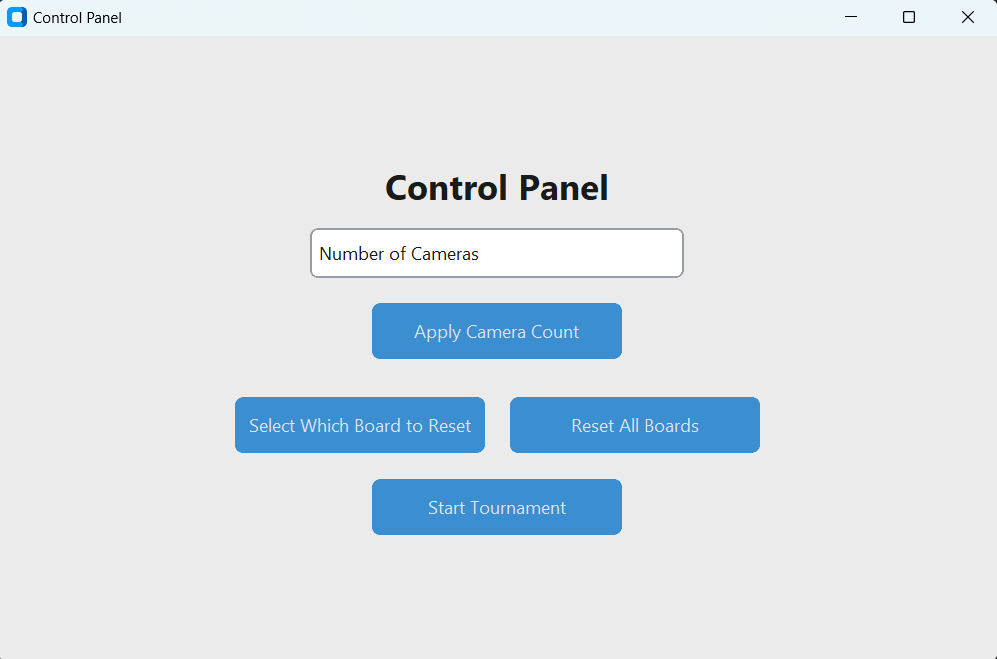
\includegraphics[width=0.75\linewidth]{figures/results/frontend/control-panel/control-panel.png} \caption[Control panel for tournament organizers]{The control panel used by the tournament organizers.}\label{fig:control-panel} \end{figure}

Once the application is launched, the accompanying web application becomes accessible to spectators. It is designed to allow viewers to follow the tournament in real time across a range of devices. Built as a responsive interface, it adapts to both desktop and mobile screens to ensure accessibility and usability. Spectators can navigate between views, observe live games, and explore additional information about the system. \\

One of the main pages in the web application is the Tournament View, which presents an overview of all ongoing games. Each entry shows the board number, the players' names and ratings, and a link to follow the game live, as shown in Figure~\ref{fig:tournament-view-mocked}. The content is updated continuously, providing spectators with a live snapshot of the tournament's progress. \\

\begin{figure}[h!] \centering \fbox{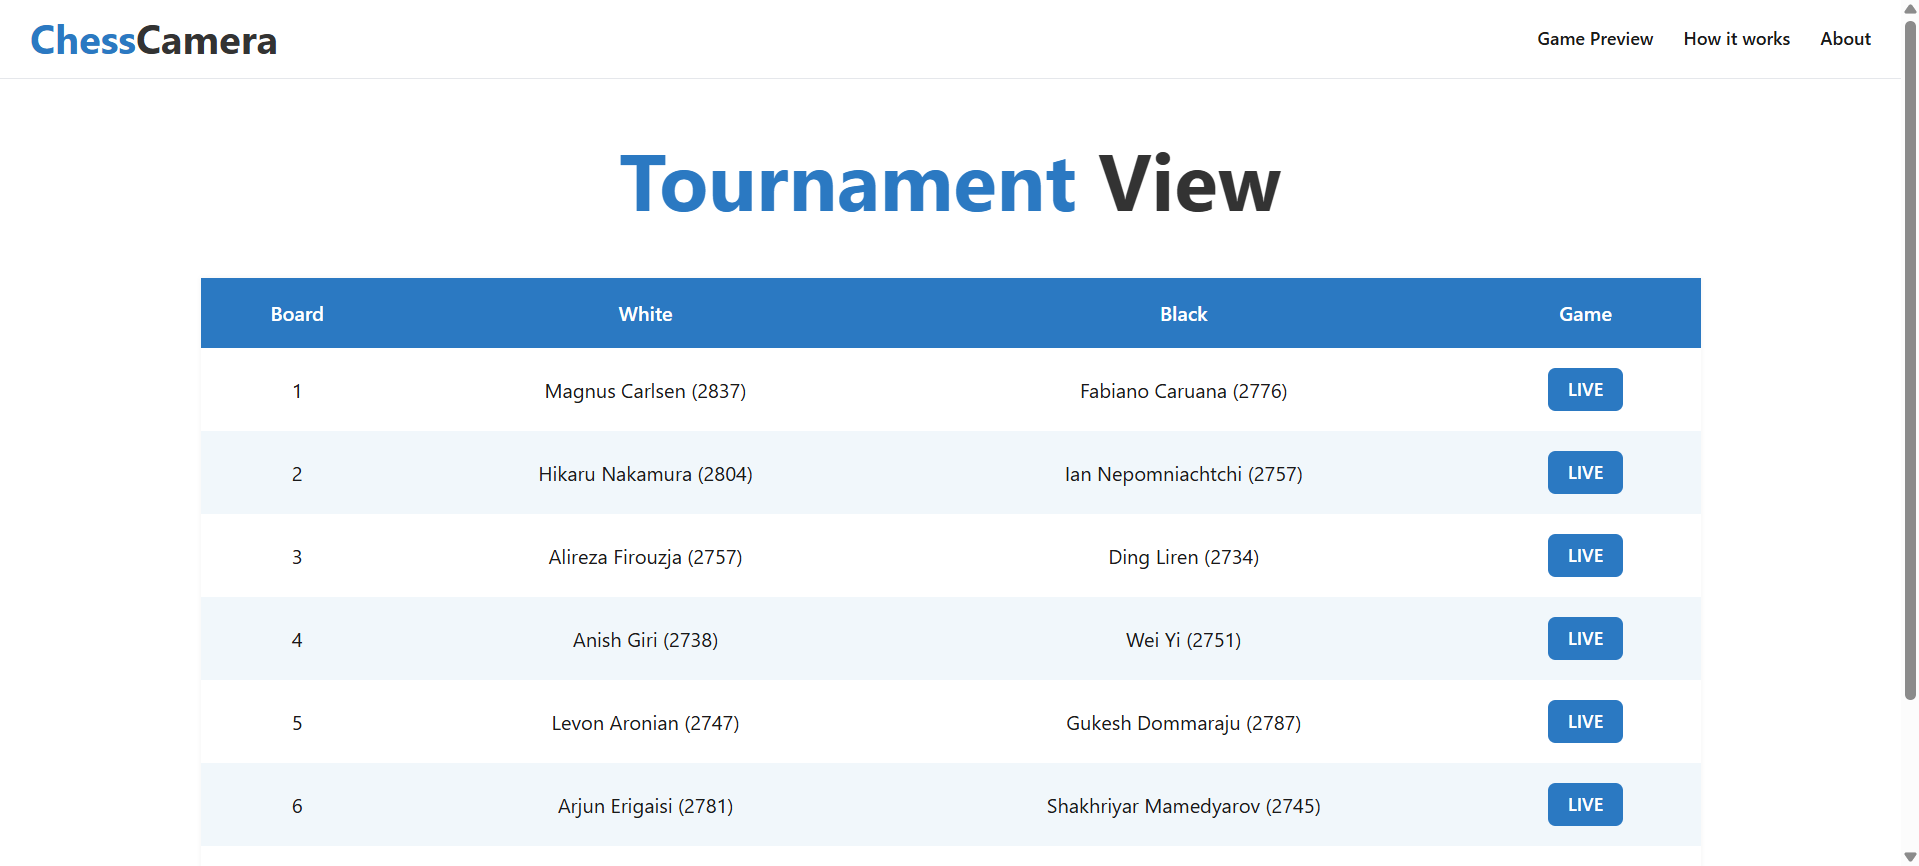
\includegraphics[width=0.75\linewidth]{figures/results/frontend/tournament-view/mocked.png}}\caption[Display of tournament]{A mocked demonstration of a tournament display.}\label{fig:tournament-view-mocked} \end{figure}

Another page is the Board View, which focuses on a single game in greater detail. This view includes a digital chessboard, a list of moves played, a live camera feed, and a visual evaluation bar, as shown in Figure~\ref{fig:board-view-mocked}. The elements update in real time, creating an engaging and intuitive experience for users following a particular match. \\

\begin{figure}[h!] \centering \fbox{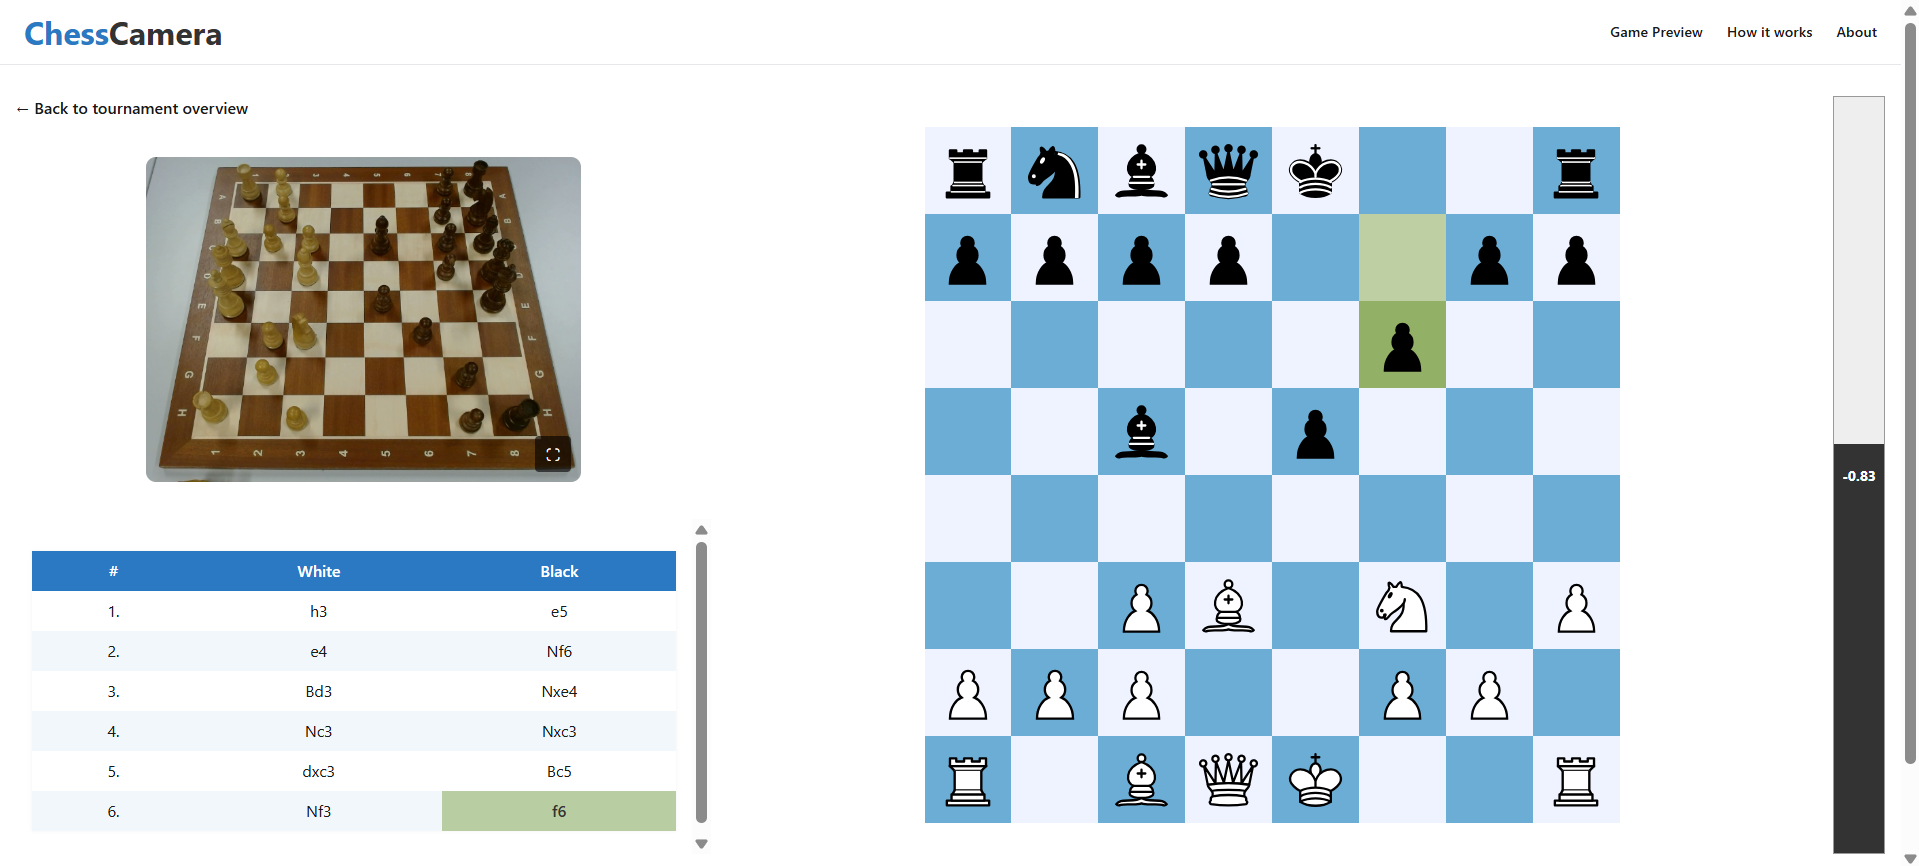
\includegraphics[width=0.75\linewidth]{figures/results/frontend/board-view/desktop.png}}\caption[Display of a board]{A mocked demonstration of an active game}\label{fig:board-view-mocked} \end{figure}

In addition, the web application features a Game Preview page that displays simplified mini-boards for multiple games. This view enables users to quickly glance through active games and select one to view in detail, as shown in Figure~\ref{fig:game-preview}. It offers a compact and efficient way to stay updated on several games at once. \\

\begin{figure}[h!] \centering \fbox{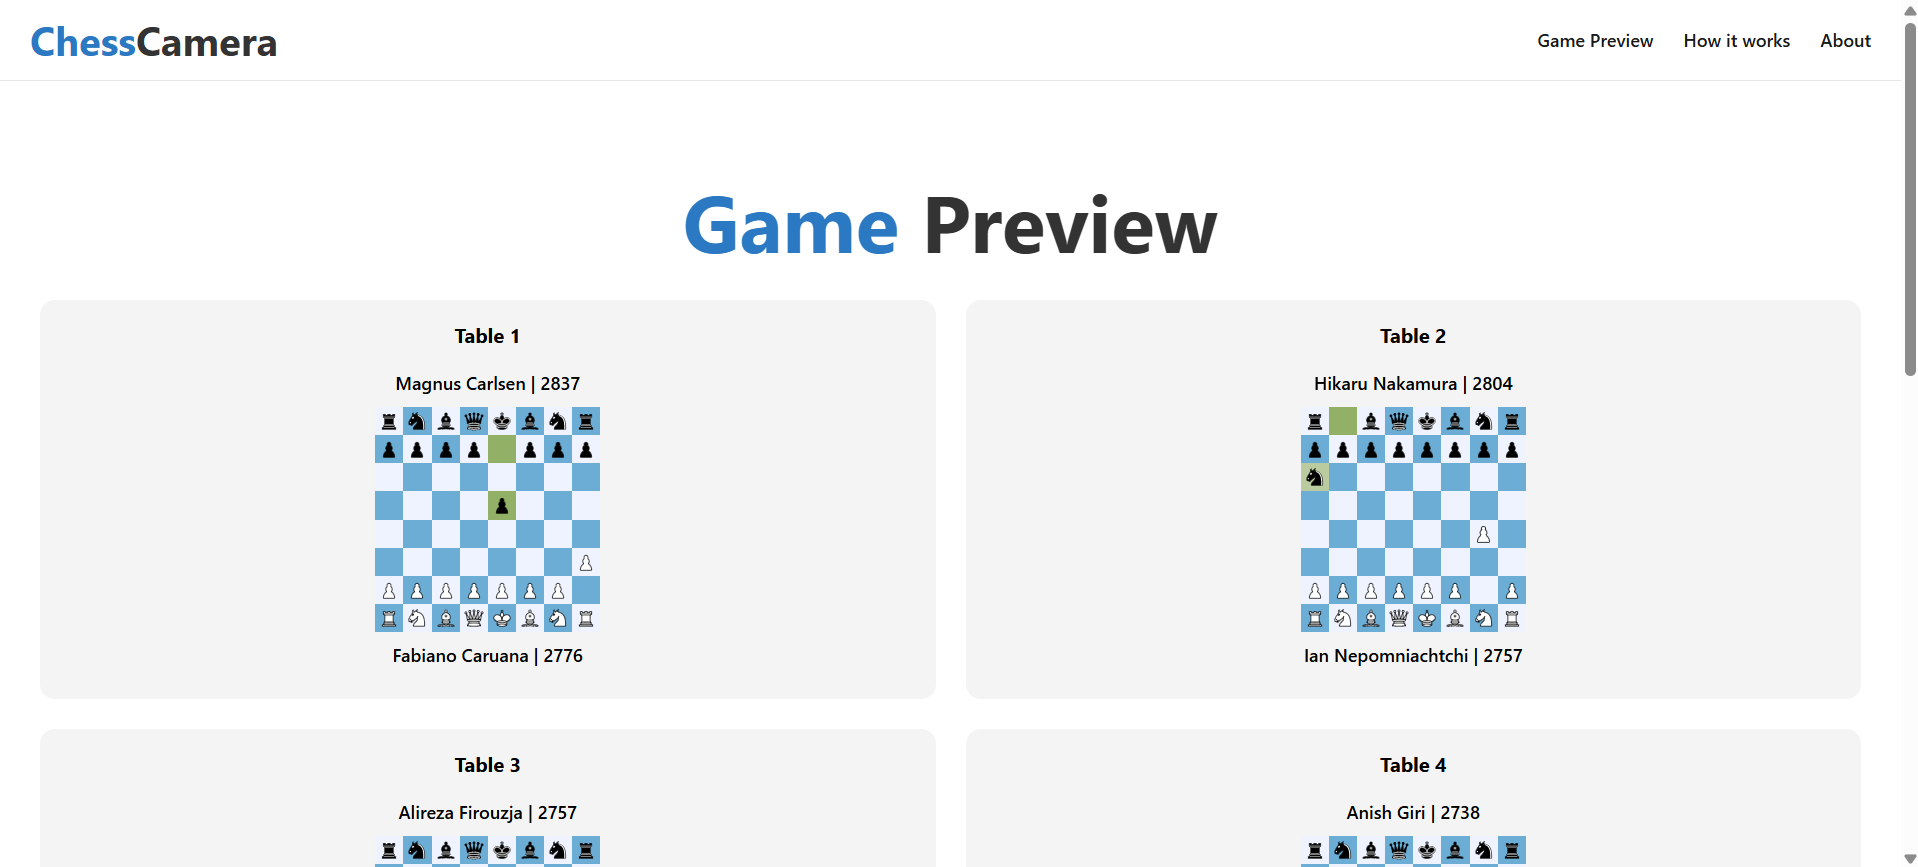
\includegraphics[width=0.75\linewidth]{figures/results/frontend/game-preview/desktop.png}}\caption[Preview of active games]{A mocked demonstration of a game preview page.}\label{fig:game-preview} \end{figure}

\section{Technical Achievements}
Architecture overview (e.g., system diagram, deployment pipeline). Performance metrics (e.g., response time, uptime). Details on scalability, security, or CI/CD if relevant. 

\section{Testing and Quality Assurance}
Summary of testing performed (unit tests, integration tests, manual testing). Test coverage results or bugs discovered/fixed. If relevant, include tables or graphs showing test results or reliability.